\documentclass[fleqn,10pt]{wlscirep}
\usepackage[utf8]{inputenc}
\usepackage[T1]{fontenc}
\usepackage[english]{babel}
\usepackage{lineno}

%\usepackage[colorlinks=true, allcolors=blue]{hyperref}
% \usepackage{physics}
\usepackage{amsmath}
\usepackage{amssymb}
\usepackage[T1]{fontenc}
\usepackage{times}
\usepackage{rotating}
\usepackage{graphicx}
\usepackage{color}
\usepackage{tensor}
\usepackage{multirow}
\usepackage[sort,numbers,round]{natbib}
\usepackage{siunitx}
\usepackage{subcaption}
\usepackage{caption}
\usepackage{textcomp}
\usepackage{url}
\usepackage{lipsum}


\definecolor{red}{rgb}{1,0,0}
\definecolor{blue}{rgb}{0,0,0.8}
\definecolor{green}{rgb}{0,0.5,0}
\newcommand{\emphc}[1]{\emph{\textcolor{red}{#1}}}
\newcommand{\emphb}[1]{\emph{\textcolor{blue}{#1}}}
\newcommand{\modif}[1]{\textcolor{green}{#1}}
\newcommand{\mean}[1]{\langle {#1} \rangle}

\newcommand{\hycom}{\textsc{hycom} }
\newcommand{\slim}{\textsc{slim}\ }
\newcommand{\ie}{{\it i.e.}\ }
\newcommand{\eg}{{\it e.g.}\ }

\linenumbers

\title{Building a model-based coral connectivity atlas of Florida’s Coral Reef}

\author[1,*]{Thomas Dobbelaere}
\author[2]{Joana Figueiredo}
\author[3]{Daniel M. Holstein}
\author[1,4]{Emmanuel Hanert}

\affil[*]{\href{mailto:thomas.dobbelaere@uclouvain.be}{thomas.dobbelaere@uclouvain.be}}
\affil[1]{Earth and Life Institute (ELI), UCLouvain, Louvain-la-Neuve, Belgium}
\affil[2]{Halmos College of Natural Sciences and Oceanography, Nova Southeastern University, Dania Beach, FL, United States}
\affil[3]{Department of Oceanography and Coastal Sciences, College of the Coast and Environment, Louisiana State University, Baton Rouge, LA, United States}
\affil[4]{Institute of Mechanics, Materials and Civil Engineering (IMMC), UCLouvain, Louvain-la-Neuve, Belgium}


\begin{abstract}
    Coral populations have experienced a world-wide decline due to both global and local anthropogenic stressors and almost all live coral cover could be lost under a >1.5°C warming. Avoiding climate change being no longer an option, local actions are required to mitigate its effects and support coral recovery. To maximize the resilience of large-scale reef systems with localized actions, knowledge about the connectivity between reefs is needed. These exchange processes are driven by currents with complex small-scale circulation features within reef systems. Hence, biophysical models that can simulate the life-traits and transport of coral larvae down to the reef scale are required to estimate coral connectivity. However, due to the important computational cost of such models, connectivity studies often consider a small number of coral species over a limited number of spawning events, therefore lacking inter-annual and inter-specific variability. Here, we used the multi-scale ocean model \slim to simulate the dispersal of larvae from 6 coral species in Florida's Coral Reef over 10 consecutive years (2012-2021). We then computed connectivity metrics to identify the reefs best suited for protection and restoration efforts over multiple years and multiple species. By identifying similar spatial patterns in connectivity measures between species, we highlight the potential for coupled restoration. Furthermore, using 10 years of modeled larval dispersal, we build robust estimates of long-term connectivity. Such estimates could be used to predict the potential evolution of the reef system and bridge the gap between genetic connectivity and larval dispersal in Florida's Coral Reef. This study provides unprecedented easy-to-access reef-scale connectivity datasets to inform the  design of future marine conservation strategies.
\end{abstract}
\begin{document}

%\begin{keyword}
%Florida reef tract \sep biophysical modeling \sep unstructured mesh ocean model \sep %coral connectivity \sep hurricane \sep ocean transport \sep stony coral tissue loss disease
%\end{keyword}

\flushbottom
\maketitle
\thispagestyle{empty}

% === INTRODUCTION ===

\section*{Introduction}

\textbf{To do: } Paragraph on The services brought by coral reefs and their worldwide decline under the combined effects of climate change and anthropogenic stressors.

As an infamous hot spot for coral disease, the Caribbean has already experienced a 50-80\% decline of live coral cover since the 1970s \citep{gardner2003long,jackson2014status}. Furthermore, the Caribbean is currently experiencing an outbreak of the stony coral tissue loss disease (SCTLD), one of the most pervasive and virulent coral diseases on record, which affects over 22 species of reef-building corals \citep{noaa2018,meiling2021variable}. This disease was first observed off the coast of Miami in 2014 \citep{precht2016unprecedented}, and has since then decimated coral populations throughout the entirety of Florida's Coral Reef (FCR) \citep{williams2021fine,frrp2021}. As a consequence, coral cover in Southeastern Florida has now dropped below 1\%, while reefs in the Florida Keys maintained a cover of roughly 6\% \citep{grove2022national}. However, extreme warm events have increased significantly in the Florida Keys in recent decades and, if trends persist, annual bleaching could occur in the region before 2034 \citep{manzello2015rapid}. Besides, Florida is a prime landfall target for tropical cyclones, which are expected to increase in intensity under climate change. It becomes thus urgent to maintain coral populations and support their recovery through restoration and conservation efforts.

\textbf{To do:} Description of conservation/restoration. As coral reef restoration is expensive and requires important man-power, it is only feasible at a limited spatial scale. Restoration sites must thus be thoughtfully selected in order to maximize the effect of restoration to the whole system. One way to inform restoration site selection is by estimating demographic connectivity, \ie~the exchanges of coral larvae between reefs. Using connectivity, outplant site can be strategically selected by identifying areas where the currents facilitate the dispersal of larvae to a greater number of surrounding reefs. 

\textbf{To do: } As larval dispersal cannot be measured empirically, estimating the exchanges of larvae between reefs require biophysical ocean models able to capture flow features down to the reef scale \citep{saint2023biophysical}. 

Such models require important computational resources and most connectivity studies cover thus a limited number of spawning events and coral species. This undermines the robustness of the derived connectivity estimates, as they lack inter-annual and interspecific variability. In this study, we simulated the dispersal of larvae from 6 coral species over 10 consecutive years (2012-2021). Using these 10 years of simulation, we identify consistent connectivity hotspots and clusters for all simulated years and species. Furthermore, by identifying pairs of coral species with strongly correlated connectivity metrics, we highlight the potential for coupled management strategies. 

% === METHODS ===

\section*{Methods}

\subsection*{Larval dispersal and connectivity modeling}

We simulated the hydrodynamics over the entirety FCR during 10 years (2012-2021) with the multiscale ocean model \slim\footnote{\href{ https://www.slim-ocean.be}{slim-ocean.be}}. This model has already been successfully validated and applied in Florida to simulate the dispersal of larvae and disease agents \citep{frys2020fine,dobbelaere2020coupled}. \slim uses an unstructured mesh whose resolution can be locally refined in order to capture flow features and tides down to the reef scale. The model mesh was generated using the seamsh\footnote{\href{https://pypi.org/project/seamsh/}{https://pypi.org/project/seamsh/}} Python library, based on the open-source mesh generator GMSH \citep{geuzaine2009gmsh}. It was made up of $6,6\times 10^5$ triangles, whose size ranged from 50 m near reefs to 13.5 km in the open sea. The mesh element size was refined based on the distance to reefs and coastlines, as well as the bathymetry and bathymetry gradient. \slim currents were relaxed towards the operational Navy HYbrid Coordinate Ocean Model (\hycom; \citealp{chassignet2007hycom}) following the approach of \citep{dobbelaere2022impacts} to capture the baroclinic dynamics of the Florida Current. Further details about the model formulation can be found in \citep{frys2020fine}.

\textcolor{red}{[insert figure of the mesh domain ?]}

The modeled currents were then used to simulate the dispersal of coral larvae using a Lagrangian particle tracker for 6 species: \textit{Acropora cervicornis} (Acer), \textit{Colpophyllia natans} (Cnat), \textit{Diploria labyrinthiformis} (Dlab), \textit{Montastrea cavernosa} (Mcav), \textit{Orbicella faveolata} (Ofav) and \textit{Pseudodiploria strigosa} (Pstr). \textcolor{red}{[insert a few sentenced explaining why we chose these particular species]}. The particle tracker implemented larvae history traits such as mortality and competence, \ie~the ability of a larvae to settle onto a reef. Mortality was either modeled using a constant mortality $\mu$ rate or a Weibull model \citep{king2023larval} with parameters $\lambda$ and $\nu$. After time to competence $t_c$, larvae were becoming competent with rate $\alpha$ and losing competence at rate $\beta$. The species-specific spawning dates and times were defined in days after the full moon (DAFM) and minutes after sunset (MAS) \textcolor{red}{[insert data source]}. Dlab spawned in April and May, Mcav in July and August, and all other coral species spawned in July and/or August. The biological and spawning parameters used in the model are summarized in Table \ref{tab:species}. 

\begin{table}
    \centering
    \small
    \begin{tabular}{lcccccccc}
        \hline
        Species & DAFM & MAS & $\mu$ & $\lambda$ & $\nu$ & $t_c$ & $\alpha$ & $\beta$ \\
                & [day] & [minute] & [hour$^{-1}$] & [hour$^{-1}$] & [-] & [hour] & [hour$^{-1}$] & [hour$^{-1}$] \\
        \hline
        Acer & 2 - 4 & 150 - 180 & - & 0.005123971 & 1.303439 & 156.0769 & 0.008409655 & 0.05612717 \\
        Cnat & 6 - 8 & 25 - 115 & - & 0.005621361 & 1.096544 & 28.20409 & 0.003140281 & 0.04740285 \\
        Dlab & 10 - 12 & -70 - 10 & 0.006276354 & - & - & 44.99998 & 0.003375632 & 0.01651378 \\
        Mcav  & 5 - 8 & 15 - 225 & - & 0.002716095 & 1.49904 & 118 & 0.002647409 & 0.0337848 \\
        Ofav & 5 - 8 & 185 - 255 & - & 0.004567343 & 1.275355 & 108 & 0.001323208 & 0.04444537 \\
        Pstr & 6 - 8 &  35 - 100, 205 - 270 & - & 0.007488953 & 1.632956, & 36.01622 & 0.02547463 & 0.1775446 \\
        \hline
    \end{tabular}
    \caption{Biological and spawning parameters used to simulate the dispersal of larvae for each modeled species: days after the full moon (DAFM), minutes after sunset (MAS), mortality rate ($\mu$), Weibull model parameters ($\lambda$,$\nu$), time to competence ($t_c$), competence acquisition ($\alpha$) and loss ($\beta$) rates. In the case of Weibull mortality, the mortality rate at larval age $t$ was given by $\lambda\nu(\lambda t)^{\nu-1}$.}\label{tab:species}
\end{table}

The reefs of Florida were extracted from the “coral reefs and hardbottom” layer of the Unified Florida Reef Tract Map \citep{fwc2017unified}. The extracted reef polygon were then further divided into 16,823 500 m $\times$ 500 m sub-reef patches to model larval exchanges at a finer scale. We assumed a uniform coral cover over all reefs, and released a total of about $10^6$ particles over all the reef polygons during each spawning simulation. Particles in the model were not representing single larvae but rather a mass of larvae, initialized at 1. Settlement of competent larval mass onto reef was occurring at deposition rate $\gamma = 0.2$ hour$^{-1}$, consistent with observed larval settling velocity \textcolor{red}{[to be confirmed]}. For each modeled spawning, the exchanges of larval mass between reefs were recorded into connectivity matrices, whose rows correspond to source reefs and whose columns correspond to destination reefs. Connectivity matrices can be more easily interpreted as large networks whose nodes are the reefs and whose edges are the larval exchanges between reefs. Connectivity metrics can then be derived from these networks using graph theory tools. The connectivity indicators used in this study are summarized in Table \ref{tab:indicators}. Finally, we identified reef clusters inside the connectivity networks using the \textit{Strongly Connected Components} (SCC) detection algorithm \citep{nuutila1994finding}. This method groups reefs in the same community if they present numerous bidirectional connections to each other, and if they are weakly connected to reefs located in other clusters. Such methods aim at identifying ecologically separated groups, hence inferring the presence of dispersal barriers between those groups \citep{thomas2014numerical,saint2023biophysical}

\begin{table}
    \centering
    \begin{tabular}{p{0.2\textwidth}p{0.45\textwidth}p{0.25\textwidth}}
        \hline
        \textbf{Indicator} & \textbf{Description} & \textbf{What it shows} \\
        \hline
        %Weighted connectivity length ($WCL_i$) & $\dfrac{\sum_{j} \tilde{C}_{ij} L_{ij}}{\sum_{j} \tilde{C}_{ij}}$ & Average dispersal distance from origin to destination reef for all particles released over a reef  \\
        Weighted out-degree & Weighted combination of the number of reefs to which a given reef sends larvae and the probability of larval export to those reefs & Reef's potential to export larvae \\
        Weighted in-degree & Weighted combination of the number of reefs from which a given reef receive larvae and the probability of larval imports from these reefs & Reef's potential to import larvae \\
        Self recruitment & Proportion of particles settling on a reef that originated from that same reef. & Reef isolation \\
        Local retention & Proportion of particles released on a given reef that settle on the same reef & Self-replenishment potential \\
        \hline
    \end{tabular}
    \caption{Connectivity indicators used to analyze the dispersal of coral larvae in the reef network.}\label{tab:indicators}
\end{table}

\subsection*{Connectivity analysis}

We estimated the similarity of the distribution of the connectivity metrics between species using the Pearson correlation coefficient following the methodology described in \citep{boccaletti2014structure}. Let $x_i^\alpha$ and $x^\beta_i$ be the connectivity metrics $x$ evaluated at node $i$ for species $\alpha$ and $\beta$, the Pearson correlation coefficient between species $\alpha$ and $\beta$ for indicator $x$ is given by:
\begin{equation}
    r_{\alpha\beta} =  \dfrac{\mean{x_i^{\alpha}x_i^{\beta}} - \mean{x_i^\alpha}\mean{x_i^\beta}}{\sqrt{\mean{x_i^\alpha x_i^\alpha} - \mean{x_i^\alpha}^2}\sqrt{\mean{x_i^\beta x_i^\beta} - \mean{x_i^\beta}^2}},
\end{equation} 
where $\mean{x_i}$ is the mean of sequence $\{x_i\}$. The value of $r_{\alpha\beta}$ ranges from -1 to 1, where 1 indicates a perfect positive correlation, 0 no correlation and -1 a perfect negative correlation.

For each species and indicator, we identified connectivity hot spots that remained consistent over the 10 simulated years. To do so, we evaluated the frequency at which the yearly value of each indicator was among the yearly top 10\% values of that indicator for all reefs. Reefs with a top 10\% frequency of 1 for a given indicator where thus found in the yearly top 10\% for that indicator every simulated year. By averaging this frequency for all species, we can identify hot spots that remained consistent for all simulated species and years for a given indicator. These species-averaged frequencies can then be multiplied to select optimal restoration sites. Such reef sites could be identified among top performers of weighted out-degree, in-degree and local retention, and low-performers of self-recruitment.

Finally, we quantified the inter-annual variability of the SCC structure for all species. This was performed by counting the number of simulated years during which any given pair of reefs was found in the same SCC. This resulted in a symmetrical matrix of shape $16,823 \times 16,823$, whose entries ranged between 0 and 10. Entries of this matrix with high values indicate pairs of reefs that were consistently found in the same SCC over the 10 simulated years. Lower values of this indicator for all reef pairs would hence infer a strong inter-annual variability of the composition of the SCCs.

% === RESULTS ===
\section*{Results}

% Indicator	Mean correlation	Standard deviation
% locRet	0.652	0.143
% wInDeg	0.901	0.054
% wOutDeg	0.792	0.090
% selfRec	0.347	0.108
% 
% Species 1	Species 2	Mean correlation
% Cnat	Pstr	0.875
% Mcav	Ofav	0.830
% Cnat	Ofav	0.754
% Cnat	Mcav	0.728
% Acer	Ofav	0.719
% Acer	Mcav	0.683
% Acer	Cnat	0.664
% Cnat	Dlab	0.658
% Ofav	Pstr	0.643
% Mcav	Pstr	0.608
% Dlab	Pstr	0.608
% Dlab	Ofav	0.599
% Dlab	Mcav	0.581
% Acer	Dlab	0.574
% Acer	Pstr	0.574

The Pearson correlation coefficients for the considered connectivity indicators and all pairs of coral species are show  in Fig. \ref{fig:correlation}. The most strongly correlated indicators were weighted in-degree and out-degree, with a species-averaged correlation factor of $0.901$ and $0.732$ respectively. Local retention, on the other hand, was the least strongly correlated indicator, with an average correlation factor of 0.347. Cnat and Pstr exhibited the most strongly correlated connectivity, with an average correlation factor of 0.875 over all considered indicators. Overall, connectivity indicators of Mcav, Cnat and Ofav, which have similar spawning windows, were more strongly correlated. On the other hand, the connectivity of Dlab, which spawns in April-May, was more weakly correlated with the other species, which spawn in July-August. Nevertheless, Acer and Pstr had the most weakly correlated connectivity indicators, with an average correlation coefficient of 0.574. This might be explained by the fact that Acer had the narrowest spawning window in terms of MAS, and Pstr the widest.

\begin{figure}
    \centering
    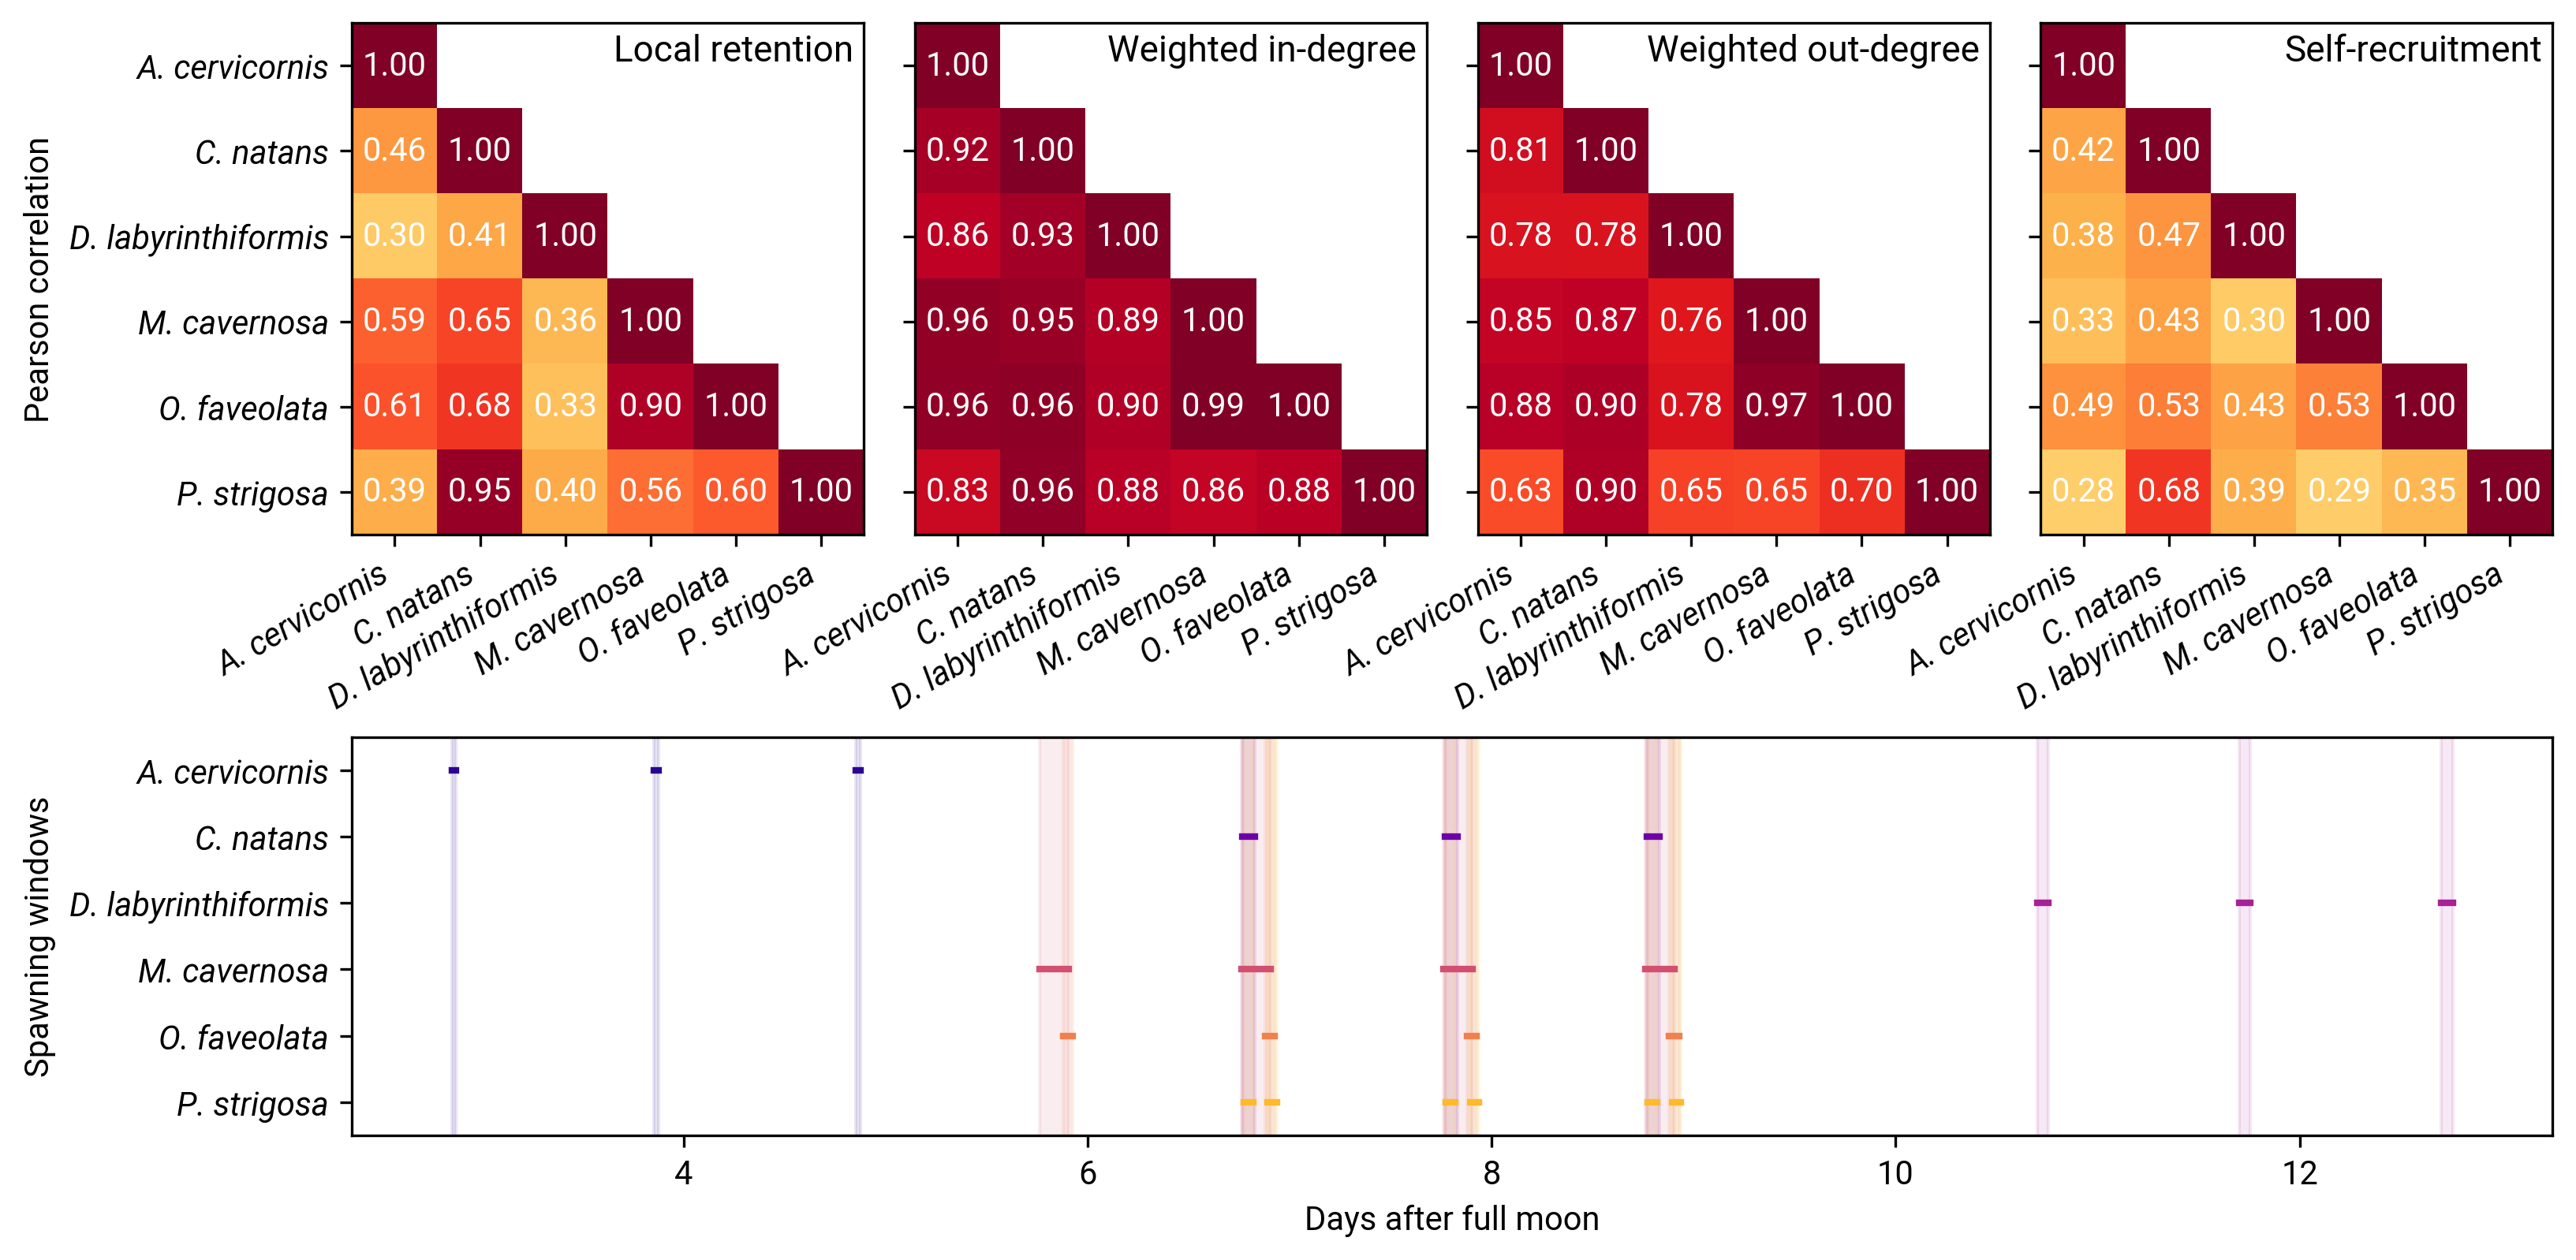
\includegraphics[width=\textwidth]{figures/fig_correlation.png}
    \caption{Pearson correlation coefficient between all pairs of species for all connectivity indicators.}\label{fig:correlation}
\end{figure}

The top-performer reefs in terms of  local retention, weigthed in-degree and weigthed out-degree are shown in Fig. \ref{fig:top10}. A cluster of top-performers in local retention is located in the region of Biscayne Bay, although reefs with a high frequency in the top 10\% can be found on offshore reefs near Key West, and in the Dry Tortugas (Fig. \ref{fig:top10}a). Top-performers in terms of weighted in-degree are pretty widespread throughout FCR, although some clusters can be found in the Upper Keys, in the inshore reefs of the Middle Keys, at the southwestern end of the Florida Keys and in the Dry Tortugas (Fig. \ref{fig:top10}b). Top-performers in terms of weighted out-degree exhibit a clearer clustering and are mostly located in the offshore reefs of the Lower and Middle Keys, as well as on the northern end of FCR (Fig. \ref{fig:top10}b). Finally, low-performers in terms of self-recruitment are mostly located in the offshore reefs of the Lower Keys and the (northern) vicinity of Biscayne Bay (Fig. \ref{fig:top10}d). When combining this information, our model identified reef with good restoration potential in the Southern Dry Tortugas, the southwestern Florida Keys, the Upper Keys and the northern end of FCR (Fig. \ref{fig:top10}e).

\begin{figure}
    \centering
    \includegraphics[width=0.9\textwidth]{figures/fig_top10_v2.png}
    \caption{Species-averaged frequency of reefs in the top 10\% yearly values for \textbf{(a)} local retention, \textbf{(b)} weighted in-degree and \textbf{(c)} weigthed out-degree. The species-averaged frequency of reefs in flop 10\% yearly values for self recruitment is shown in panel \textbf{(d)}. By multiplying these frequencies, we obtain a combined restoration indicator whose top values correspond to reefs that are top performers of weighted out-degree, in-degree and local retention, and low-performers of self-recruitment, as shown in panel \textbf{(e)}. Reefs with value 0 of the quantity highlighted in each panel are shown in black}\label{fig:top10}
\end{figure}

The structure and composition of the SCCs evolved through time for each simulated species (Fig. \ref{fig:scc}). Ofav, Acer and Mcav exhibited the least stable SCC structure, as they yield the weakest number of reef pairs found in the same SCC during all 10 simulated year, with Ofav having the least stable SCC structure. On the other hand, the largest number of reef pairs found in the same SCC during all 10 simulated years was observed in the connectivity network of Ofav. This suggests that this species had the most stable SCC structure. A comparison of the SCC composition of Ofav and Dlab in 2015 and 2016 is shown in Fig. \ref{fig:scc}. While most of the SCC structure is conserved between those two years for Ofav, strong structural differences are observed for Dlab, especially in the Middle Keys and the Dry Tortugas. Finally, for all modeled species, reefs with IDs $5000$ to $10,000$, where often found in the same SCC during several simulated years. This corresponds to reefs located in the Middle and Upper Keys. This suggests that reefs of these areas tend to be strongly connected to each other for all species. 

\begin{figure}
    \centering
    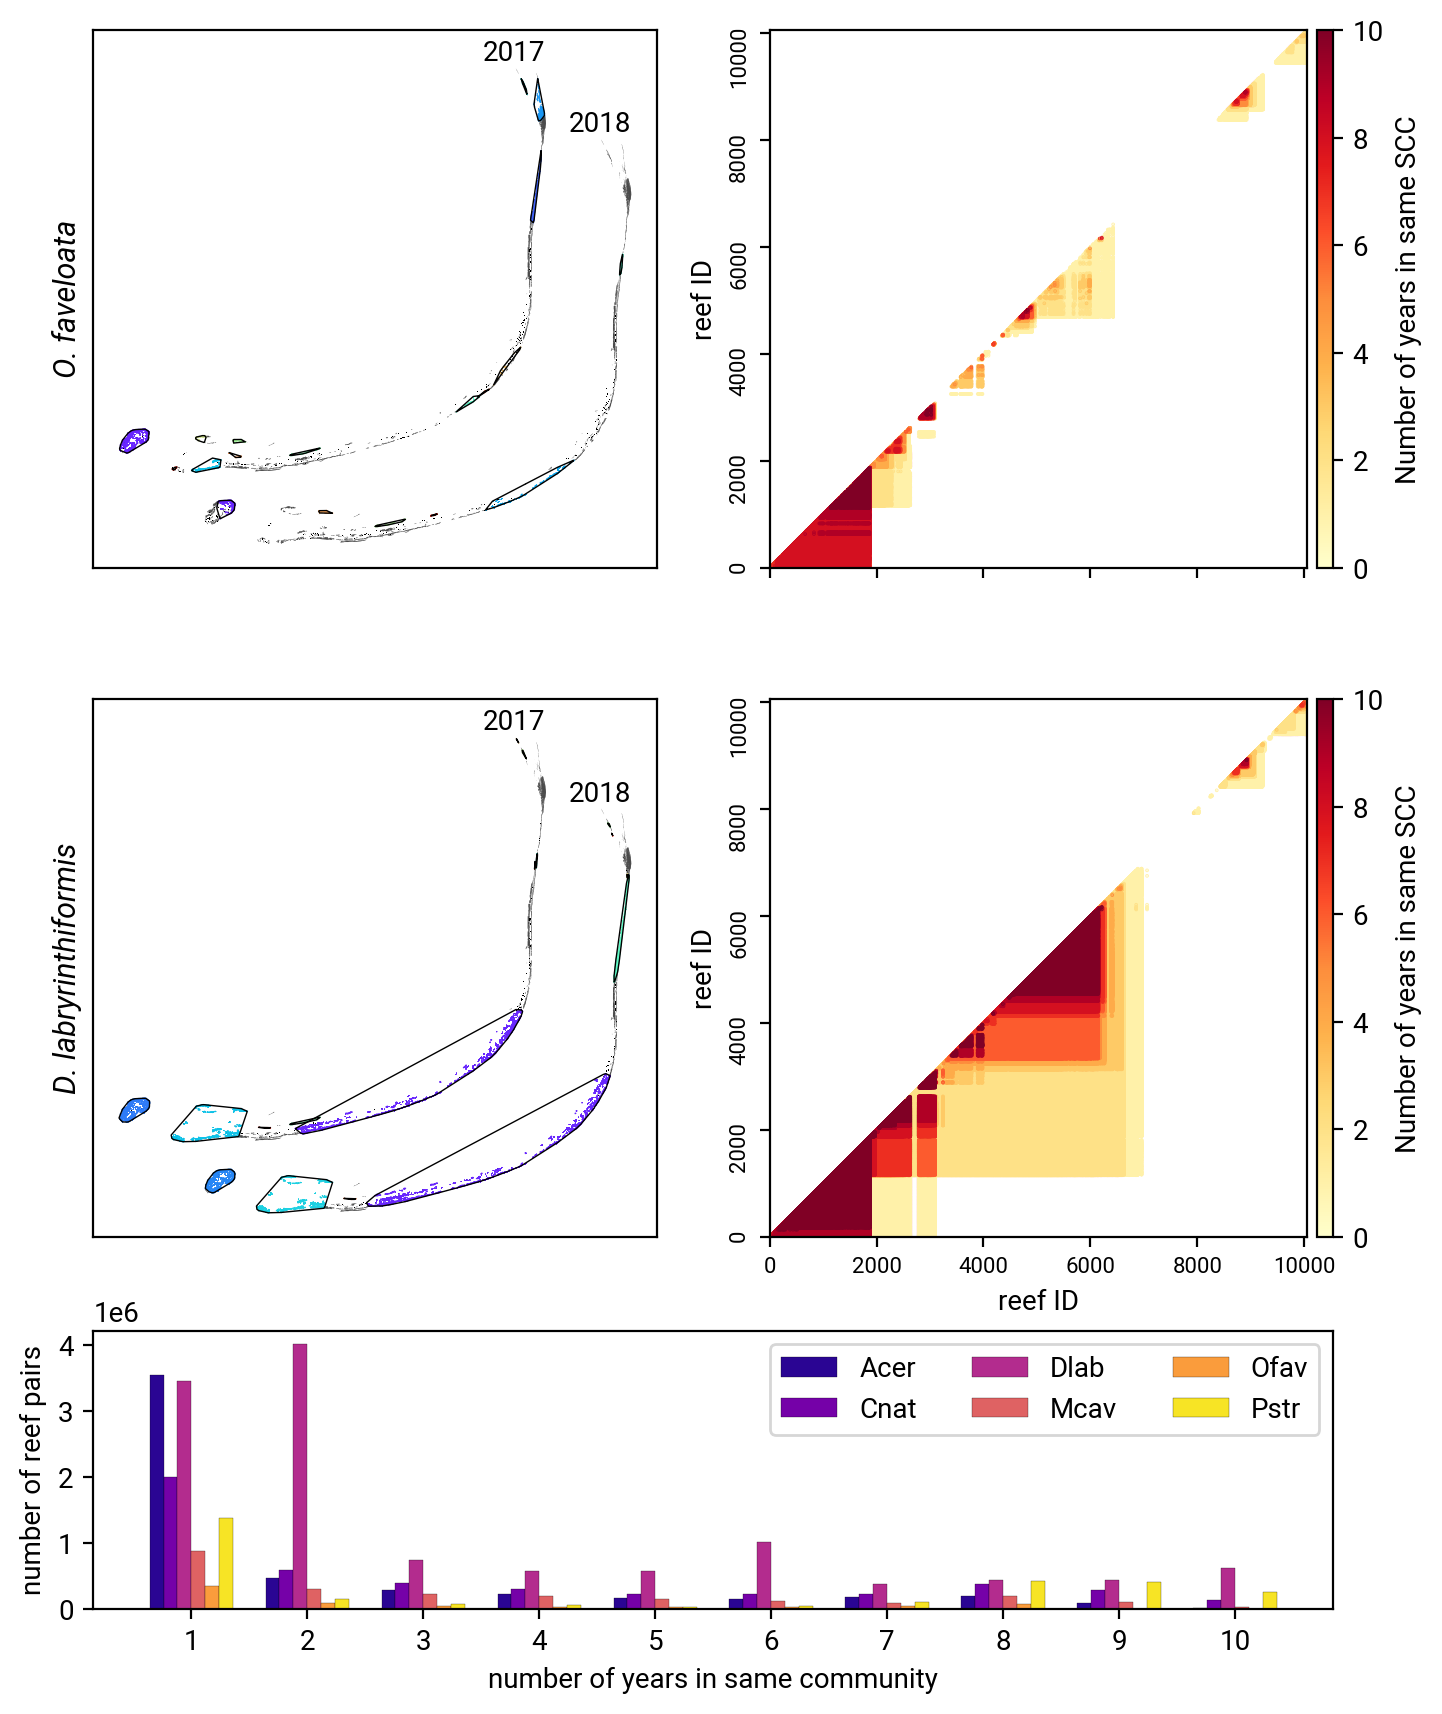
\includegraphics[width=\textwidth]{figures/comparison_sccs.png}
    \caption{SCCs of the connectivity networks of Ofav (\textbf{top}), and Dlab (\textbf{middle}) in 2015 and 2016, and the symmetrical matrix counting the number of simulated years during which each pair of reefs was found in the same SCC for these 2 species. \textbf{Bottom}: Number of reef pairs found in the same SCC vs. the number of simulated years during which they were found in the same community for each modeled coral species.}\label{fig:scc}
\end{figure}

% === DISCUTION ===

\section*{Discussion}

\textbf{Paragraph idea:} Summary of the results

\textbf{Paragraph idea:} Potential for coupled restoration

\textbf{Paragraph idea:} The importance of inter-annual variability of the connectivity indicators (based on results of Fig. \ref{fig:scc}) \textcolor{red}{add Fig. \ref{fig:variabibility} to results ?}

\textbf{Paragraph idea:} Importance of robust connectivity estimates to optimize coral restoration in regard of climate change. 

\textbf{Paragraph idea:} Limitations of the study: 2D model $+$ Potential connectivity $\rightarrow$ habitat suitability and post-settlement survival not considered $+$ we assumed an uniform coral cover over all reefs by lack of 
information

\begin{figure}
    \centering
    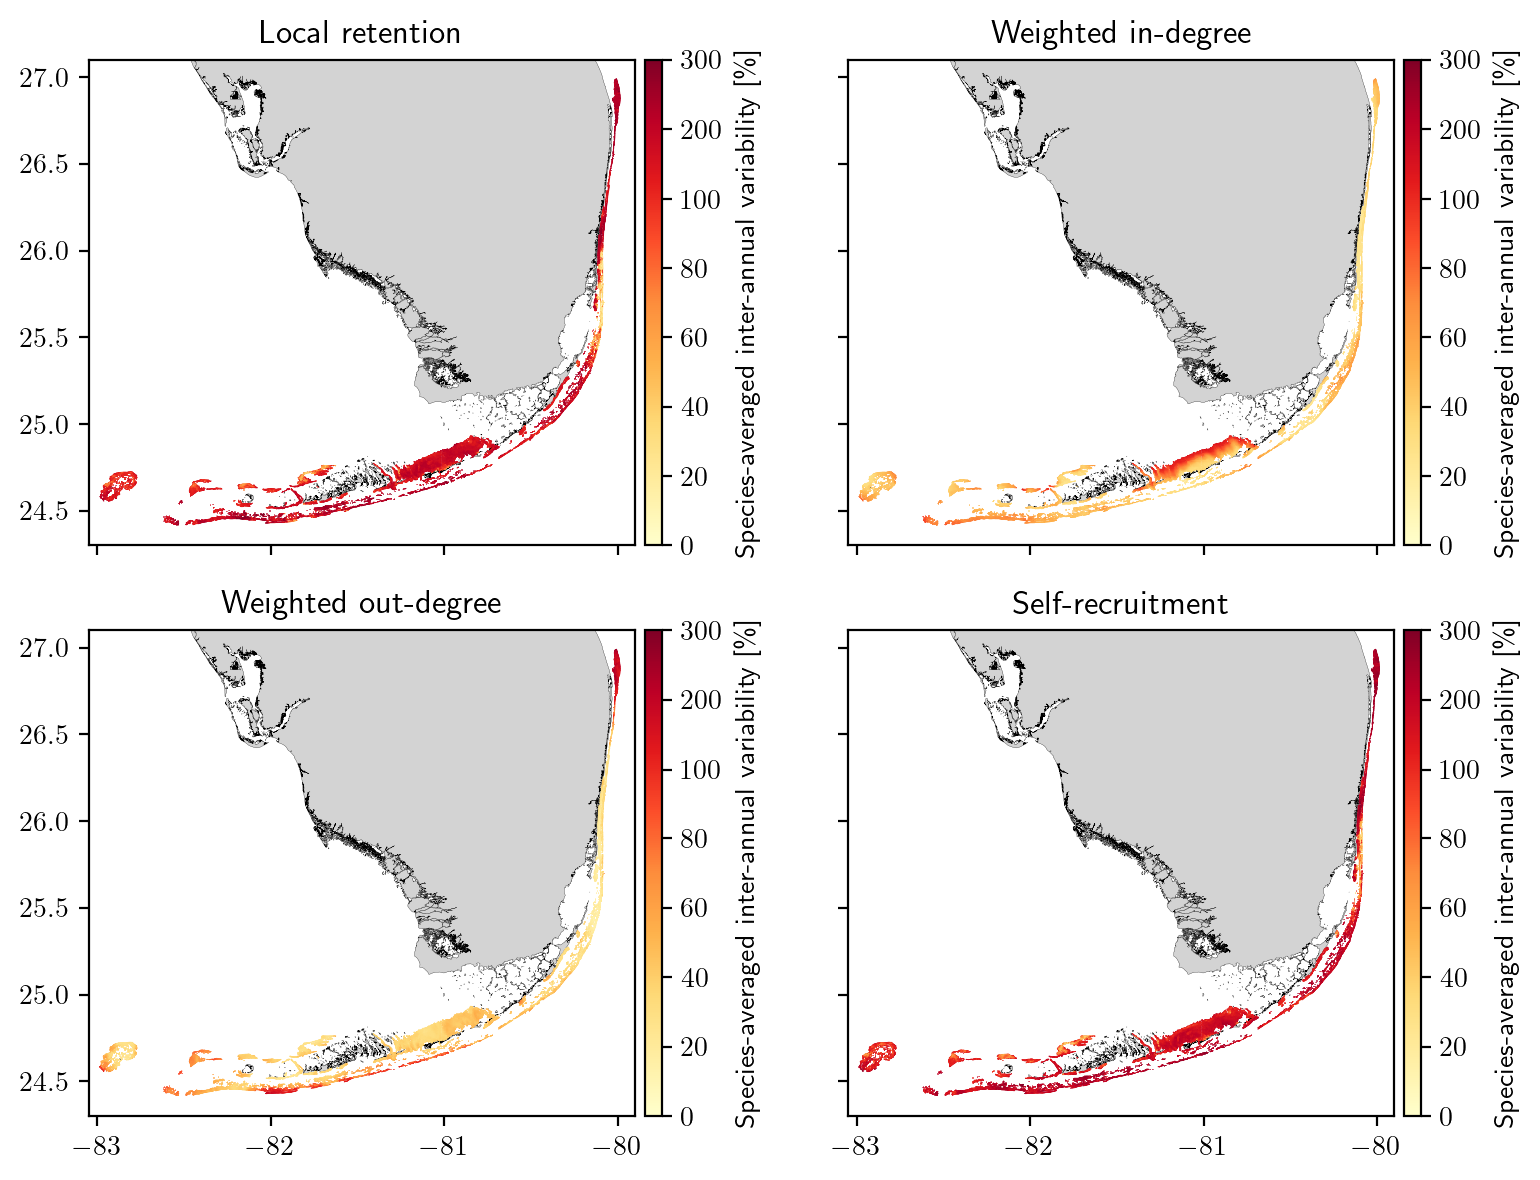
\includegraphics[width=\textwidth]{figures/fig_std.png}
    \caption{\textcolor{red}{[Additional result ?]} Species-averaged standard deviation of the reef value of all connectivity indicators, expressed as a percentage of the yearly-averaged reef value.}\label{fig:variabibility}
\end{figure}
% === CONCLUSION ===

\section*{Conclusion}

\lipsum[1-1]

% === Lots of stuff ===

\section*{Data availability}

TBD.
% The datasets generated during the current study are available from the corresponding author on reasonable request.

\section*{Code availability}

The \slim source code can be found at \href{https://git.immc.ucl.ac.be/slim/slim}{https://git.immc.ucl.ac.be/slim/slim}.


\section*{Acknowledgements}

Computational resources have been provided by the supercomputing facilities of the \it{Universit\'e catholique de Louvain} (CISM/UCLouvain) and the \it{Consortium des \'Equipements de Calcul Intensif en F\'ed\'eration Wallonie Bruxelles} (CECI) funded by the \it{Fonds de la Recherche Scientifique de Belgique} (F.R.S.-FNRS) under convention 2.5020.11.

\section*{Author contributions statement}
TBD. 

\section*{Competing interests}
The authors declare no competing interests.

% === REFERENCE ===

\bibliography{biblio.bib}

\end{document}